\documentclass[a5paper,14pt]{report}
\usepackage{amsmath}
\usepackage{amssymb}
\usepackage[english, russian]{babel}
%\usepackage[cp1251]{inputenc}
\usepackage[T1,T2A]{fontenc} %added
\usepackage[utf8]{inputenc}
\usepackage[dvips]{graphicx}
\graphicspath{{images/}}
\usepackage{indentfirst}
\usepackage{multicol}
\usepackage{hhline}
\usepackage{multirow}
\usepackage{textcomp}
\usepackage{wrapfig}
\usepackage{color,colortbl}
\definecolor{Gray1}{gray}{0.7}
\definecolor{Gray2}{gray}{0.6}
\definecolor{Gray3}{gray}{0.5}
\definecolor{Gray4}{gray}{0.4}
\usepackage{geometry}
\geometry{left=1.5cm}
\geometry{right=1.5cm}
\geometry{top=1cm}
\geometry{bottom=2cm}
\newcommand*{\hm}[1]{#1\nobreak\discretionary{}{\hbox{$\mathsurround=0pt #1$}}{}}


\begin{document}

\begin{titlepage}
Балакшин П.В., Соснин В.В.  Информатика. – СПб: Университет ИТМО, 2018. – 122 с.
\\\\\textbf{TO REVIEW AND REWRITE!!!!} В пособии излагаются основные понятия, необходимые для более глубокого изучения компьютерной техники и систем в будущем. Рассматриваются основные принципы построения, функционирования и организации памяти ЭВМ. Предлагается изучить несколько пакетов, в том числе систему компьютерной верстки TeX, и некоторые варианты распознавания того, что данные были переданы с ошибкой.
\\\\\\\\Рекомендовано к печати Ученым советом факультета программной инженерии и компьютерной техники. 
\vspace{5 cm}
\begin{flushright}

\includegraphics[width=5cm]{ITMO_log}
\end{flushright}
Университет ИТМО – ведущий вуз России в области информационных и фотонных технологий, один из немногих российских вузов, получивших в 2009 году статус национального исследовательского университета. С 2013 года Университет ИТМО – участник программы повышения конкурентоспособности российских университетов среди ведущих мировых научно-образовательных центров, известной как проект «5 в 100». Цель Университета ИТМО – становление исследовательского университета мирового уровня, предпринимательского по типу, ориентированного на интернационализацию всех направлений деятельности. 
\begin{flushright}
\copyright Университет ИТМО, 2018
\\\copyright Балакшин П.В., Соснин В.В., 2018
\end{flushright}
\end{titlepage}

\tableofcontents

\newpage
%\textbf{О курсе\\}
\section{О курсе}

Цель данного методического пособия состоит в изучении общих принципов работы компьютера и получении навыков работы с рядом пакетов. Студентам предлагается рассмотреть для получения базовых знаний и умений по работе с компьютером такие темы как: 
\begin{itemize}

\item основы теории информации;
\item сжатие компьютерных данных;
\item помехоустойчивое кодирование;
\item архитектура ЭВМ;
\item организация компьютерных сетей;
\item работа с офисными пакетами;
\item программное обеспечение профессионального программиста.
\end{itemize}

Наряду с этими темами, авторы этого пособия предоставляют возможность более детально ознакомиться с рядом современных пакетов, в их числе такие широко известные продукты Microsoft, как Microsoft Office Word и Microsoft Excel, и система компьютерной верстки TeX, имеющая свой собственный язык разметки. Освоение указанных пакетов позволит студентам получить полезные навыки по подготовке презентаций, научно-технических отчетов о результатах выполненной работы, в оформлении результатов исследований в виде статей и докладов на научно-технических конференциях. Также авторы пособия продемонсрируют не-которые методики использования программных средств для решения практических задач.


\newpage
%\textbf{Введение в информатику\\}
\section{Терминология информатики}

Начать изучение информатики невозможно, не разобравшись в точном значении термина «информатика». Однако, до сих пор в мировой научной общественности не сложилось четкого понимания этого термина. Рассмотрим одно из популярных определений:

\textbf{Информатика} – дисциплина, изучающая свойства и структуру информации, закономерности ее создания, преобразования, накопления, передачи и использования. За рубежом сложилась чуть более узкая трактовка термина информатика. Там под этим понимают пересечение сразу трех областей науки – это информационные технологии, теория информации и computer science. Всё обозначенное выше подходит под определение самого курса "Информатика".

Изучая некоторую науку важно представлять основные даты, вехи её развития:
\begin{itemize}
\item 1956(57) – появление термина «информатика» (\textit{нем.} Informatik, Штейнбух).
\item 1968 – первое упоминание в СССР (информология, Харкевич).
\item 197Х – информатика стала отдельной наукой.
\item 4 декабря – день российской информатики.
\end{itemize}

\newpage
%\textbf{Основы теории информации\\}
\section{Терминология теории информации}

Рассмотрим некоторые терминологические тонкости. В обыденном языке, слова <<информация>> и <<данные>> считаются синонимами. Они, как правило, употребляются взаимозаменяемо. И так обстоит дело в информатике и в целом, в компьютерных науках.



Понятие \textit{"информация"} имеет различные трактовки в различных предметных областях. Например,\textit{информация} может пониматься как:
\begin{itemize}
\item сигналы для управления, приспособления рассматриваемой системы (в кибернетике);
\item мера хаоса в рассматриваемой системе (в физике);
\item вероятность выбора в рассматриваемой системе (в теории вероятностей);
\item мера разнообразия в рассматриваемой системе (в биологии) и др.
\end{itemize}
 Но мы остановимся на понятиях, близких к информатике.
\\
\\\textbf{Информация} - это некоторая упорядоченная последовательность сообщений, отражающих, передающих и увеличивающих наши знания.
\\
\\\textbf{Информация} - это сведения об окружающем мире (объекте, процессе, явлении, событии), которые являются объектом преобразования (включая хранение, передачу и т.д.) и используются для выработки поведения, для принятия решения, для управления или для обучения.
\\
\\\textbf{Информация} - это новые сведения, подлежащие передаче, хранению и обработке.s
\newpage 
Рассмотрим это фундаментальное понятие информатики на основе понятия \textit{"алфавит"} ("алфавитный", формальный подход). Дадим формальное определение \textit{алфавита}.
\\
\\\textbf{Алфавит} - конечное множество различных знаков (букв), символов, для которых определена операция \emph{конкатенации} (присоединения символа к символу или цепочке символов); с ее помощью по определенным правилам соединения символов и слов можно получать слова (цепочки знаков) и словосочетания (цепочки \textit{слов}) в этом \textit{алфавите} (над этим \textit{алфавитом}).
\\
\\\textbf{Знак (буква)} - любой элемент алфавита (элемент $x$ алфавита $X$, где $x \in X$). Понятие знака неразрывно связано с тем, что им обозначается ("со смыслом"), они вместе могут рассматриваться как пара элементов ($x$, $y$), где $x$ – сам знак, а $y$ – обозначаемое этим знаком.\\
\\\emph{\textbf{Пример 1:}}
\\Примеры \emph{алфавитов:} множество из десяти цифр, множество из знаков русского языка, точка и тире в азбуке Морзе и др. В \emph{алфавите} цифр знак 5 связан с понятием "быть в количестве пяти элементов".\\
\\\textbf{Слово} в алфавите (или над алфавитом) - конечная последовательность знаков (букв) алфавита.
\\
\\\textbf{Длина} |p| некоторого слова $p$ в алфавите (над алфавитом) - число составляющих его букв.
\\
\\\textbf{Словарь (словарный запас)} - множество различных слов в алфавите (над алфавитом).
\\В отличие от конечного \emph{алфавита}, словарный запас может быть и бесконечным.\\
\\\emph{Слова} над некоторым заданным \emph{алфавитом} и определяют так называемые \emph{сообщения}.\\
\\\emph{\textbf{Пример 2:}}
\\\emph{Слова} над \emph{алфавитом} кириллицы - "Информатика","инто", "ииии'', "и". 
\\\emph{Слова} над \emph{алфавитом} десятичных цифр и знаков арифметических операций – "1256", "23+78", "35–6+89", "4". 
\\\emph{Слова} над \emph{алфавитом} азбуки Морзе – ".", ". . –", "– – –".\\
\\В  \emph{алфавите} должен быть определен порядок следования \emph{букв} (порядок типа "предыдущий элемент – последующий элемент"), то есть любой \emph{алфавит} имеет упорядоченный вид $X = {x_1, x_2, …, x_n}$ .\\
\\Таким образом, \emph{алфавит} должен позволять решать задачу лексикографического (алфавитного) упорядочивания, или задачу расположения \emph{слов} над этим \emph{алфавитом}, в соответствии с порядком, определенным в \emph{алфавите} (то есть по символам \emph{алфавита}).

\section{Признаки классификации информации}

Рассмотрим две классификации информации. Первая из них - классификация по форме \emph{сообщений} - определенного вида сигналов, символов:
\begin{itemize}
  \item отношение к источнику или приемнику (входная, выходная и внутренняя);
  \item отношение к конечному результату (исходная, промежуточная и результирующая);
  \item актуальность;
  \item адекватность;
  \item доступность (открытая, закрытая);
  \item понятность;
  \item полнота (достаточная, недостаточная, избыточная);
  \item достоверность;
  \item массовость;
  \item изменчивость (постоянная, переменная, смешанная);
  \item объективность;
  \item точность;
  \item стадия использования (первичная, вторичная);
  \item ценность.
\end{itemize}

Вторая классификация - по форме преставления информации, способам ее кодирования и хранения:
\begin{itemize}
  \item графическая;
  \item звуковая;
  \item текстовая;
  \item числовая;
  \item видеоинформация.
\end{itemize}

\section{Измерение количества информации}
Любые сообщения измеряются в \emph{байтах, килобайтах, мегабайтах, гигабайтах, терабайтах, петабайтах} и \emph{эксабайтах}, а кодируются, например, в компьютере, с помощью \emph{алфавита} из нулей и единиц, записываются и реализуются в ЭВМ в \emph{битах}.

Приведем основные соотношения между единицами измерения \emph{сообщений}:
\begin{itemize}
\item 1 бит (\textbf{bi}nary digi\textbf{t} - двоичное число) = 0 или 1;
\item 1 байт = 8 бит;
\item 1 килобайт (1Кб) = $2^{13}$ бит;
\item 1 мегабайт (1Мб) = $2^{23}$ бит;
\item 1 гигабайт (1Гб) = $2^{33}$ бит;
\item 1 терабайт (1Тб) = $2^{43}$ бит;
\item 1 петабайт (1Пб) = $2^{53}$ бит;
\item 1 эксабайт (1Эб) = $2^{63}$ бит.
\end{itemize}

Теперь нам известно понятие информации, но необходимо еще конкретно знать сколько этой информации. Поэтому есть два важных определения:
\\
\\\textbf{Количество информации} - число, адекватно характеризующее разнообразие (структурированность, определённость,выбор состояний и т.д.) в оцениваемой системе. Количество информации часто оценивается в битах, причем такая оценка может выражаться и в долях бит (так как речь идет не об измерении или кодировании сообщений).
\\
\\\textbf{Мера информации} - численная оценка количества информации, которая обычно задана неотрицательной, определенной на множестве событий и являющейся аддитивной функцией (то есть, мера информации объединения событий (множеств) равна сумме мер каждого события). Заметим, что функция меры информации монотонна (при уменьшении или увеличении вероятности некоторого события количество иноформации в системе монотонно уменьшается или увеличивается). 
\\\textbf{Важно:} мера вероятности всегда находится в диапазоне от 0 до 1.
\par
Для измерения информации используются различные подходы и методы, например, с использованием меры информации по Р. Хартли и К. Шеннону.

\newpage
\subsection{Мера Хартли}

\begin{wrapfigure}{l}{2.7cm}
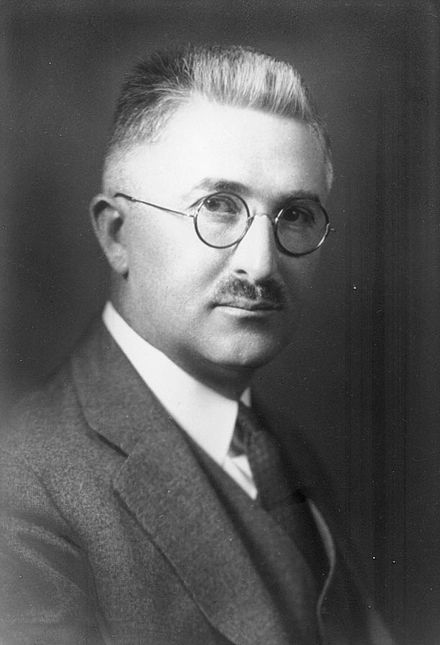
\includegraphics[width=2.7cm]{4_3_1}
\begin{center}
\footnotesize{Ральф Хартли}
\\\footnotesize{$1888 - 1970$}
\end{center}
\end{wrapfigure}

Пусть известны $N$ состояний системы $S$ ($N$  опытов с различными, равновозможными, последовательными состояниями системы). Если каждое состояние системы закодировать двоичными кодами, то минимальная длина $d$ полученного кода определяется из условия:

$$2^{d} \ge N \qquad \mbox{\emph{или}} \qquad  d \ge \log_{2}N$$
Значит, для однозначного описания системы требуется $\log_{2}N$ бит. В общем случае количество информации в системе $S$ равно:
$$H_{s} = \log_{k}N$$
Единицы измерения количества информации:
\begin{itemize}
  \item Бит ($k = 2$)
  \item Трит ($k = 3$)
  \item Дит (харт) ($k = 10$)
  \item Нит (нат) ($k = e$)
\end{itemize}
\begin{center}
\textbf{Примеры использования меры Хартли}
\end{center}
\emph{\textbf{Пример 1:}}
\\\emph{Задание:} мальчик загадывает число от 1 до 64. Какое количество вопросов типа "да-нет" понадобится, чтобы гарантированно угадать число?
\\\emph{Решение:}
\\$\bullet$ Первый вопрос: "Загаданное число меньше 32?". Ответ: "Да".
\\$\bullet$ Второй вопрос: "Загаданное число меньше 16?". Ответ: "Нет".
\\ \dots
\\$\bullet$ Шестой вопрос точно приведет к правильному ответу.
\\
\\Значит, в соответствии с мерой Хартли в загадке мальчика содержится $\log_{2}64 = 6$ бит информации ($N = 64$ так как возможно 64 вариантов загаданного числа).
\\Ответ: 6 бит.
\\
\\\emph{\textbf{Пример 2:}}
\\\emph{Задание:} мальчик держит за спиной шахматного ферзя и собирается поставить его на произвольную клетку пустой доски. Какое количество информации содержится в его действии?
\\\emph{Решение:} шахматная доска имеет размеры $8\times 8$ клеток. Ферзь может быть как белым, так и черным, поэтому количество равновероятных состояний будет равно $8\times 8 \times 2 = 128$. Получается, количество информации по мере Хартли равно $\log_{2}128 = 7$ бит.
\\Ответ: 7 бит.
\\Если во множестве $X = {x_1,x_2, ..., x_n}$ искать произвольный элемент, то для его нахождения (по Хартли) необходимо иметь не менее $\log_{a}n$ (единиц) информации. 
\\Уменьшение $Н$ говорит об уменьшении разнообразия состояний $N$ системы, увеличение $Н$ говорит об увеличении разнообразия состояний $N$ системы.
\\
\\Мера Хартли подходит лишь для идеальных, абстрактных систем, так как в реальных системах состояния системы неодинаково осуществимы (неравновероятны).

\subsection{Мера Шеннона }
\begin{wrapfigure}[12]{l}{2.5cm}
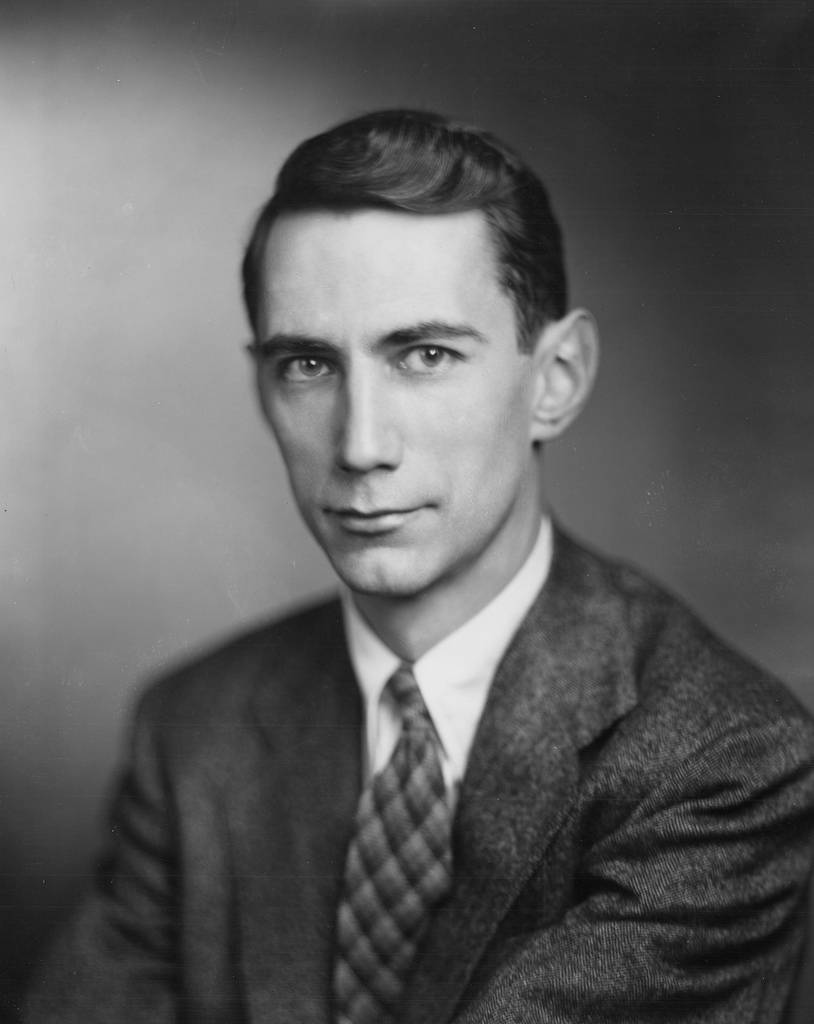
\includegraphics[width=2.5cm]{4_3_2}
\begin{center}
\footnotesize{Клод Шеннон}
\\\footnotesize{$1916 - 2001$}
\end{center}
\end{wrapfigure}

Если состояния системы не равновероятны, используют меру Шеннона. Мера Шеннона оценивает информацию отвлеченно от ее смысла:
$$I = - \sum^{N}_{i=1}p_{i}\times \log_{2}p_{i},$$ где:
\\$I$ - количество информации, выраженное в битах (в $\log_{k}p_{i}$ $k = 2$);
\\$N$ - число состояний системы;
\\$p_{i}$ - вероятность (относительная частота) перехода системы в $i$-е состояние (вероятность того, что система находится в состоянии $i$) \\Сумма всех $p_{i}$ должна быть равна единице.\\
\\Если все состояния рассматриваемой системы равновозможны, равновероятны, то есть $р_i = 1/n$ , то из \emph{формулы Шеннона} можно получить (как частный случай) \emph{формулу Хартли}:
$$I = \log_{2}n.$$
\\Обозначим величину:
$$f_i = -n\log_{2}p_i.$$
\newpage
Тогда из \emph{формулы К. Шеннона} следует, что количество информации I можно понимать как среднеарифметическое величин $f_i$ , то есть величину $f_i$ можно интерпретировать как \emph{информационное содержание символа алфавита} с индексом i и величиной $p_i$ вероятности появления этого символа в любом сообщении (слове), передающем информацию.\\
\\ В термодинамике известен так называемый коэффициент Больцмана $k = 1.38 * 10^{-16} (эрг.град)$ и выражение (\emph{формула Больцмана}) для энтропии или меры хаоса в термодинамической системе:
$$ S = -k \sum^{N}_{i=1}p_{i}\times \ln{p_{i}}$$
\\ Сравнивая выражения для I и S, можно заключить, что величину I можно понимать как энтропию из-за нехватки информации в системе (о системе).\\
\\Формулы энтропии и информации идентичны, но смысл разный. Энтропия априорная характеристика (до передачи), информация – апостериорная (после передачи).\\
\\Из этой формулы следуют важные выводы:
\begin{itemize}
\item увеличение меры Шеннона свидетельствует об уменьшении энтропии (увеличении порядка) системы;
\item уменьшение меры Шеннона свидетельствует об увеличении энтропии (увеличении беспорядка) системы.
\end{itemize}
Положительная сторона \emph{формулы Шеннона} – ее отвлеченность от смысла информации. Кроме того, в отличие от \emph{формулы Хартли}, она учитывает различность состояний, что делает ее пригодной для практических вычислений. Основная отрицательная сторона \emph{формулы Шеннона} – она не распознает различные состояния системы с одинаковой вероятностью.

\begin{center}
\textbf{Примеры использования меры Шеннона}
\end{center}
\emph{\textbf{Пример 1:}}
\\\emph{Задание:} девочка наугад вытаскивает из мешка мяч. Известно, что в мешке всего 8 мячей, из них: 4 красных, 2 синих, 1 зеленый и 1 белый. Какое количество информации содержится в этом событии?
\\\emph{Решение:}
\\$\bullet$ Вероятность вытащить красный мяч равна $^4/_8 = 0,5$
\\$\bullet$ Вероятность вытащить синий мяч равна $^2/_8 = 0,25$
\\$\bullet$ Вероятность вытащить зеленый мяч равна $^1/_8 = 0,125$
\\$\bullet$ Вероятность вытащить белый мяч равна $^1/_8 = 0,125$
\\Значит количество информации, выраженное в битах равно: $I = -(0,5\hm\times \log_{2}0,5\hm + 0,25\hm\times \log_{2}0,25 + 0,125\hm\times \log_{2}0,125\hm + 0,125\hm\times \log_{2}0,125) \hm = -(-0,5\times 1 - 0,25\times 2 - 0,125\times 3 - 0,125\times 3) = -(-0,5 - 0,5\hm - 0,375\hm - 0,375\hm) = 1,75$ бит.
\\Ответ: 1,75 бит

\section{Методы получения информации}
Методы получения информации можно разбить на три большие группы:
\begin{itemize}
\item \emph{Эмпирические};
\item \emph{Теоретические}; 
\item \emph{Эмпирико-теоретические}.
\end{itemize}
Кратко рассмотрим и охарактеризуем все три метода по отдельности. 
\subsection{Эмпирические методы}
\emph{Эмпирические методы или методы получения эмпирических данных.}
\begin{enumerate}
\item \emph{Наблюдение} -- сбор первичной информации об объекте, процессе, явлении.
\item \emph{Сравнение} -- обнаружение и соотнесение общего и различного.
\item \emph{Измерение} -- поиск с помощью измерительных приборов эмпирических фактов.
\item \emph{Эксперимент} -- преобразование, рассмотрение объекта, процесса, явления с целью выявления каких-то новых свойств.
\end{enumerate}
Кроме классических форм их реализации, в последнее время используются опрос, интервью, тестирование и другие.
\subsection{Теоретические методы}
\emph{Теоретические методы или методы построения различных теорий.}
\begin{enumerate}
\item \emph{Восхождение от абстрактного к конкретному} -- получение знаний о целом или о его частях на основе знаний об абстрактных проявлениях в сознании, в мышлении.
\item \emph{Идеализация} -- получение знаний о целом или его частях путем представления в мышлении целого или частей, не существующих в действительности.
\item \emph{Формализация} -- получение знаний о целом или его частях с помощью языков искусственного происхождения (формальное описание, представление).
\item \emph{Аксиоматизация} -- получение знаний о целом или его частях с помощью некоторых аксиом (не доказываемых в данной теории утверждений) и правил получения из них (и из ранее полученных утверждений) новых верных утверждений.
\item \emph{Виртуализация} -- получение знаний о целом или его частях с помощью искусственной среды, ситуации.
\end{enumerate}

\subsection{Эмпирико-теоретические методы}
\emph{Эмпирико-теоретические методы (смешанные) или методы построения теорий на основе полученных эмпирических данных об объекте, процессе, явлении.}
\begin{enumerate}
\item \emph{Абстрагирование} -- выделение наиболее важных для исследования свойств, сторон исследуемого объекта, процесса, явления и игнорирование несущественных и второстепенных.
\item \emph{Анализ} -- разъединение целого на части с целью выявления их связей.
\item \emph{Декомпозиция} -- разъединение целого на части с сохранением их связей с окружением.
\item \emph{Синтез} -- соединение частей в целое с целью выявления их взаимосвязей.
\item \emph{Композиция} -- соединение частей целого с сохранением их взаимосвязей с окружением.
\item \emph{Индукция} -- получение знания о целом по знаниям о частях.
\item \emph{Дедукция} -- получение знания о частях по знаниям о целом.
\item \emph{Эвристики, использование эвристических процедур} -- получение знания о целом по знаниям о частях и по наблюдениям, опыту, интуиции, предвидению.
\item \emph{Моделирование (простое моделирование)}, использование приборов -- получение знания о целом или о его частях с помощью модели или приборов.
\item \emph{Исторический метод} -- поиск знаний с использованием предыстории, реально существовавшей или же мыслимой.
\item \emph{Логический метод } -- поиск знаний путем воспроизведения частей, связей или элементов в мышлении.
\item \emph{Макетирование} -- получение информации по макету, представлению частей в упрощенном, но целостном виде.
\item \emph{Актуализация} -- получение информации с помощью перевода целого или его частей (а следовательно, и целого) из статического состояния в динамическое состояние.
\item \emph{Визуализация} -- получение информации с помощью наглядного или визуального представления состояний объекта, процесса, явления.
\end{enumerate}
Кроме указанных классических форм реализации теоретико-эмпирических методов часто используются и мониторинг (система наблюдений и анализа состояний), деловые игры и ситуации, экспертные оценки (экспертное оценивание), имитация (подражание) и другие формы.\\
\\\emph{\textbf{Пример :}}
\\Для построения модели планирования и управления производством в рамках страны, региона или крупной отрасли нужно решить следующие проблемы:
\begin{enumerate}
\item определить структурные связи, уровни управления и принятия решений, ресурсы; при этом чаще используются методы наблюдения, сравнения, измерения, эксперимента, анализа и синтеза, дедукции и индукции, эвристический, исторический и логический методы, макетирование и др.;
\item определить гипотезы, цели, возможные проблемы планирования; наиболее используемые методы – наблюдение, сравнение, эксперимент, абстрагирование, анализ, синтез, дедукция, индукция, эвристический, исторический, логический и др.;
\item конструирование эмпирических моделей; наиболее используемые методы – абстрагирование, анализ, синтез, индукция, дедукция, формализация, идеализация и др.;
\item поиск решения проблемы планирования и просчет различных вариантов, директив планирования, поиск оптимального решения; используемые чаще методы – измерение, сравнение, эксперимент, анализ, синтез, индукция, дедукция, актуализация, макетирование, визуализация, виртуализация и др.
\end{enumerate}


%\chapter{Единицы измерения объема данных}
%\input {chapter1}
%
%\chapter{Системы счисления}
%\input {chapter2}
%
%\chapter{Арифметика в ограниченной разрядной сетке}
%\input {chapter3}
%
%\chapter{Теория информации}
%\input {chapter4}
%
%\chapter{Сжатие данных}
%\input {chapter5}
%
%\chapter{Помехоустойчивое кодирование}
%\input {chapter6}
%
%\chapter{Алгебра логики}
%\input {chapter7}
%
%\chapter{Программное обеспечение}
%\input {chapter8}
%
%\chapter{Структура и принципы функционирования компьютера}
%\input {chapter9}
%
%\chapter{Организация хранения данных в ЭВМ}
%\input {chapter10}
%
%\chapter{Передача данных в компьютерных сетях}
%\input {chapter11}

\end{document} 